\documentclass[10pt,a4paper]{article}
\usepackage[T1]{fontenc}
\usepackage[a4paper,margin=1.8cm]{geometry}
\usepackage{xcolor,booktabs,tabularx,array,enumitem,graphicx}
\usepackage[hyphens]{url}
\usepackage[colorlinks=true,linkcolor=black,urlcolor=black]{hyperref}

\definecolor{blk}{HTML}{C0392B}
\definecolor{ask}{HTML}{D68910}
\definecolor{fre}{HTML}{1E8449}
\newcommand{\HOOK}{\colorbox{ask!20}{\textcolor{ask}{\textbf{\strut HOOK}}}}
\newcommand{\HARN}{\colorbox{blk!20}{\textcolor{blk}{\textbf{\strut HARNESS}}}}
\newcommand{\RULE}{\colorbox{fre!20}{\textcolor{fre}{\textbf{\strut RULE}}}}
\newcommand{\p}[1]{\nolinkurl{#1}}
\newcolumntype{L}{>{\raggedright\arraybackslash}X}
\setlist{nosep,leftmargin=*}
\setlength{\parindent}{0pt}
\renewcommand{\arraystretch}{1.25}

\title{Claude Code setup: overview}
\author{\texttt{\textasciitilde/.claude} @ \texttt{a6f9d83} + uncommitted}
\date{2026-10-30}

\begin{document}
\maketitle

\noindent\textbf{Goal.} Claude works the way a careful collaborator would: it plans and waits for approval before any
change, never creates branches or worktrees by surprise, keeps a terse map of each repo current, and leaves handoff
notes so a fresh session can resume. This report shows the pieces that make that happen; the sandbox has its own
report in \p{../sandbox/sandbox-structure.pdf}.

\noindent\textbf{Enforcement legend.}
\HARN\ enforced by Claude Code itself \quad
\HOOK\ enforced by one of the hooks below \quad
\RULE\ instruction in \p{CLAUDE.md} only (Claude follows it; nothing checks).

\medskip
\begin{center}
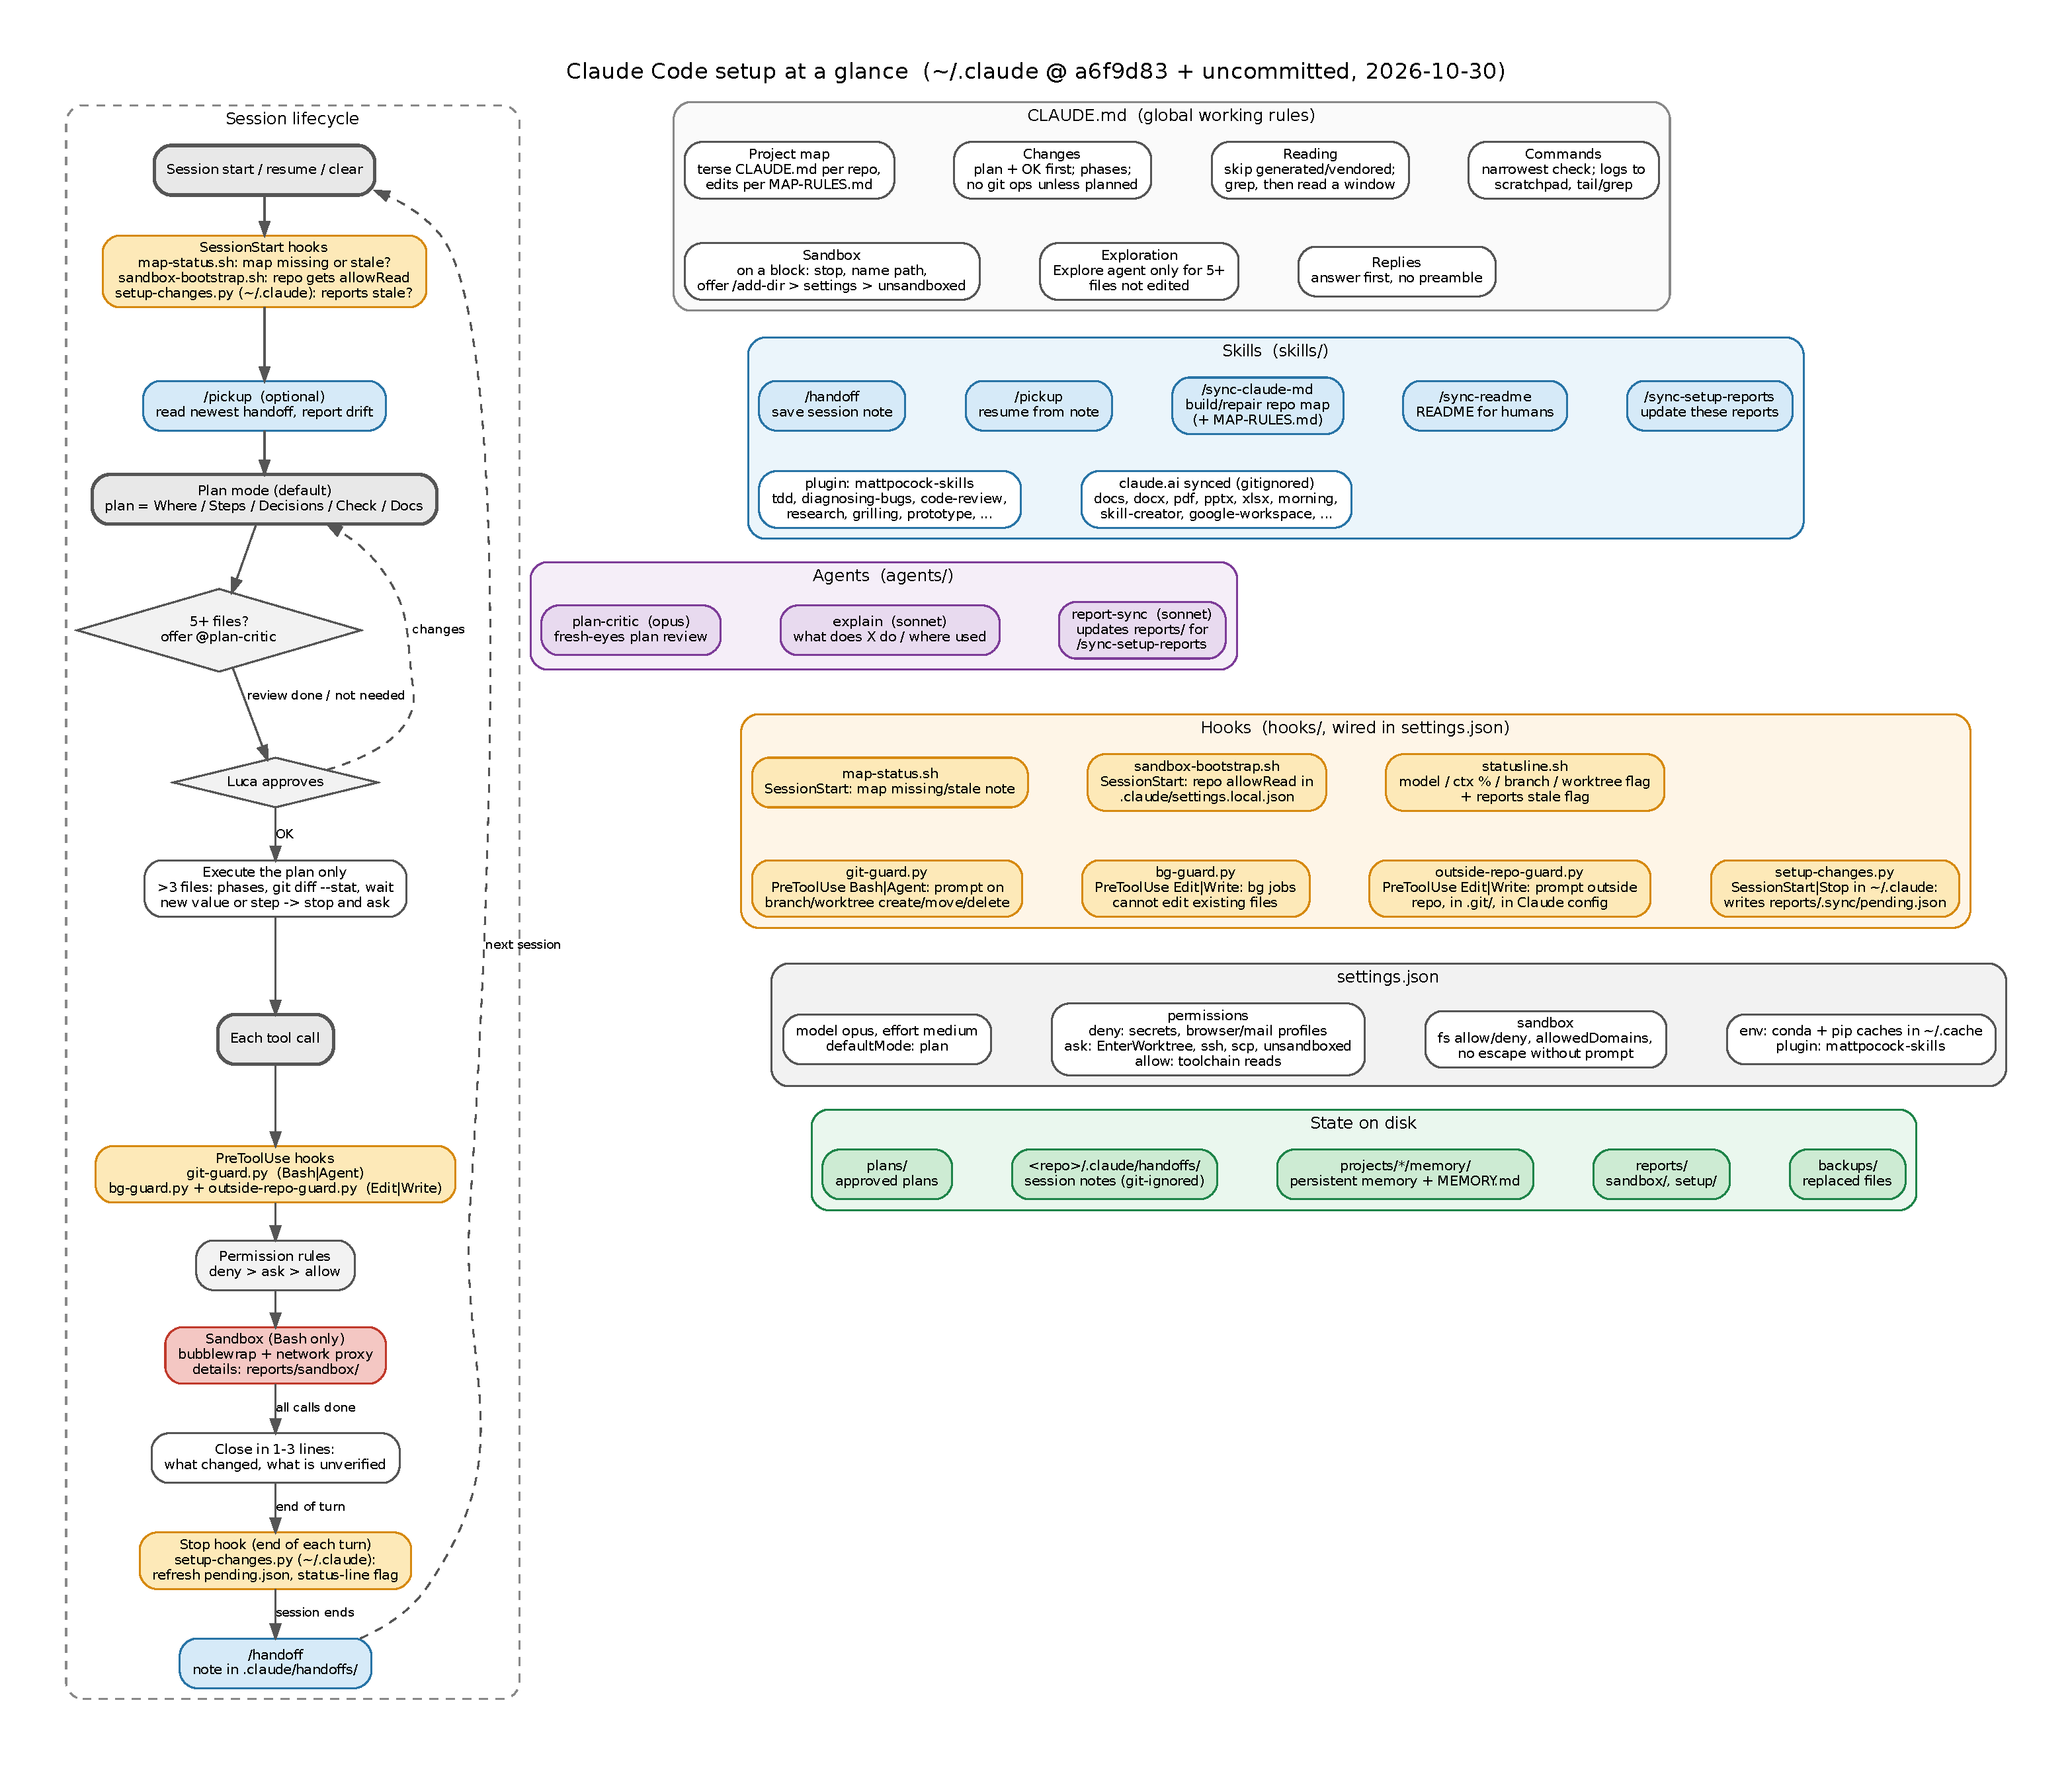
\includegraphics[width=\linewidth,height=0.72\textheight,keepaspectratio]{setup-flow.pdf}
\end{center}
\clearpage

\section{Working rules (\texttt{CLAUDE.md})}
Global instructions loaded in every session.

\begin{tabularx}{\linewidth}{@{}l L >{\raggedright\arraybackslash}p{4.3cm}@{}}
\toprule
\textbf{Section} & \textbf{Rule} & \textbf{Enforced by} \\
\midrule
Project map & Each repo has a terse \p{CLAUDE.md} map; trust it, flag it when stale, edit it by
  \p{skills/sync-claude-md/MAP-RULES.md}. Never applied in \p{~/.claude} itself. & \HOOK\ \p{map-status.sh} + \RULE \\
Changes & Plan first (Where / Steps / Decisions / Check / Docs) and wait for OK; every chosen value listed;
  $>$3 files in phases; 5+ files: offer \p{@plan-critic}; no branch, commit, push, stash unless planned. &
  \HARN\ plan mode + \HOOK\ \p{git-guard.py} + \RULE \\
Reading & Skip generated and vendored files; in large files \p{grep -n}, then read a window. & \RULE \\
Commands & Narrowest check first, full suite once; noisy output to a log, then \p{tail}/\p{grep}; quiet modes. & \RULE \\
Sandbox & On a block, stop and name the path or host; offer \p{/add-dir}, then a settings edit,
  then an unsandboxed retry. Never work around it. & \HARN\ sandbox + \HOOK\ \p{outside-repo-guard.py} \\
Exploration & Explore subagent only when 5+ files would be read and not edited. & \RULE \\
Replies & Answer first, no preamble; after changes close in 1--3 lines. & \RULE \\
\bottomrule
\end{tabularx}

\section{Skills}
Invoked as \p{/name}. Own skills have \p{disable-model-invocation}: they run only when typed.

\begin{tabularx}{\linewidth}{@{}l l L@{}}
\toprule
\textbf{Skill} & \textbf{Source} & \textbf{What it does} \\
\midrule
\texttt{/handoff [focus]} & own & Saves the session (goal, state, decisions, open questions, next step, pointers) as a note
  in \p{<repo>/.claude/handoffs/}. \\
\texttt{/pickup [slug]} & own & Reads a handoff and its pointers, compares with git now (branch, commits, uncommitted files),
  reports in $\le$5 lines, waits. \\
\texttt{/sync-claude-md [path]} & own & Builds or repairs a repo's \p{CLAUDE.md} map: draft, OK, write.
  Rules in \p{MAP-RULES.md}. Runs in the main session (a fork would inherit plan mode). \\
\texttt{/sync-readme [path]} & own & Builds or refreshes a \p{README.md} for human readers, with research sections and a fork
  rule: draft, OK, write. \\
\texttt{/sync-setup-reports} & own & Updates these reports after setup changes: lists the changed files, runs the
  \p{report-sync} agent, shows the diff for review, then stamps the snapshot on OK. \\
\midrule
mattpocock-skills & plugin & \p{tdd}, \p{diagnosing-bugs}, \p{code-review}, \p{research}, \p{grilling},
  \p{prototype}, \p{domain-modeling}, \p{codebase-design}, \p{pr}, \p{wizard}, \p{writing-for-agents}. \\
claude.ai synced & account & \p{docs}, \p{docx}, \p{pdf}, \p{pptx}, \p{xlsx}, \p{morning}, \p{skill-creator},
  \p{google-workspace}, \p{import-memory}, \dots\ In \p{skills/synced/}, git-ignored, refreshed by sync. \\
\bottomrule
\end{tabularx}

\section{Agents}
Subagents in \p{agents/}. \p{explain} and \p{plan-critic} are read-only (Read, Grep, Glob): they can look, never change.

\begin{tabularx}{\linewidth}{@{}l l L@{}}
\toprule
\textbf{Agent} & \textbf{Model} & \textbf{When it is used} \\
\midrule
\p{explain} & sonnet & ``What does X do / how does X work / where is X used'' about code not yet read in the session.
  Cheaper model; the answer comes back as a summary. \\
\p{plan-critic} & opus & Fresh-eyes review of a plan before approval: on request, or offered for plans touching 5+ files. \\
\p{report-sync} & sonnet & Used only by \p{/sync-setup-reports}: updates \p{reports/} from \p{reports/.sync/pending.json}
  and rebuilds them. Tools: Read, Grep, Glob, Edit, Write, Bash. \\
\bottomrule
\end{tabularx}

\section{Hooks}
Scripts in \p{hooks/}, wired in \p{settings.json}. A PreToolUse hook can let a call through, force a prompt, or deny it.

\begin{tabularx}{\linewidth}{@{}l l L@{}}
\toprule
\textbf{Event (matcher)} & \textbf{Script} & \textbf{Effect} \\
\midrule
SessionStart (startup, clear) & \p{map-status.sh} & Tells Claude when the repo has no map, or when $\ge$3 source files or any
  manifest changed since the map's verified commit. \\
SessionStart (startup, resume, clear) & \p{sandbox-bootstrap.sh} & Adds the repo to \p{allowRead} in its
  \p{.claude/settings.local.json} (the sandbox denies \p{~/} by default) and keeps that file out of git. \\
SessionStart (startup, resume, clear), Stop & \p{setup-changes.py} & In \p{~/.claude} only: compares the setup files with the
  snapshot of the last report sync and writes the difference to \p{reports/.sync/pending.json}. \\
PreToolUse (Bash, Agent) & \p{git-guard.py} & Forces a prompt before creating, moving or deleting a branch or worktree,
  and for Agent \p{isolation: worktree}. \\
PreToolUse (Edit, Write, NotebookEdit) & \p{bg-guard.py} & In a background job (\p{$CLAUDE_JOB_DIR} set): denies edits to
  existing files outside the job dir, temp dirs and memory. New files stay allowed. \\
PreToolUse (Edit, Write, NotebookEdit) & \p{outside-repo-guard.py} & Forces a prompt for edits outside the repo, inside
  \p{.git/}, or to Claude's own hooks, settings, skills, agents, \p{CLAUDE.md}. \\
statusLine & \p{statusline.sh} & Model $\cdot$ context used $\cdot$ git branch, flagged inside a linked worktree, and in \p{~/.claude} when the reports are stale (\p{pending.json} exists). \\
\bottomrule
\end{tabularx}

\section{Settings (\texttt{settings.json})}
\begin{tabularx}{\linewidth}{@{}l L@{}}
\toprule
\textbf{Key} & \textbf{Value} \\
\midrule
Model & \p{opus}, effort \p{medium}. \\
\p{defaultMode} & \p{plan}: every session starts read-only until a plan is approved. \\
Permissions & \textbf{deny} Read/Edit of secrets (\p{~/.ssh}, \p{~/.gnupg}, keyrings, \p{pwd.txt}, credentials) and
  browser/mail profiles and caches; \textbf{ask} \p{EnterWorktree}, \p{ssh}, \p{scp}, unsandboxed Bash;
  \textbf{allow} reads of toolchain dirs (conda, caches, Jupyter, Mathematica, MATLAB, TeX, Rust, \dots). \\
Sandbox & Bubblewrap around Bash, network allow-list, no escape without a prompt. Full rules:
  \p{../sandbox/sandbox-structure.pdf}. \\
Env & \p{CONDA_PKGS_DIRS}, \p{PIP_CACHE_DIR} in \p{~/.cache} (writable inside the sandbox). \\
Plugins & \p{mattpocock-skills}. \\
Theme & \p{dark-daltonized}. \\
\bottomrule
\end{tabularx}

\section{State and files}
\begin{tabularx}{\linewidth}{@{}l L@{}}
\toprule
\textbf{Where} & \textbf{What} \\
\midrule
\p{plans/} & Approved plans, one file per plan (tracked). \\
\p{<repo>/.claude/handoffs/} & Handoff notes from \p{/handoff}, read by \p{/pickup}; git-ignored globally. \\
\p{projects/*/memory/} & Persistent memory per project, indexed by \p{MEMORY.md}. \\
\p{reports/} & This report (\p{setup/}) and the sandbox report (\p{sandbox/}). \p{reports/.sync/} (git-ignored): snapshot of the
  setup at the last sync and \p{pending.json}. \\
\p{backups/} & Copies of files replaced during setup. \\
\p{.gitignore} & Whitelist: tracks only \p{CLAUDE.md}, \p{settings.json}, \p{agents/}, \p{hooks/}, \p{skills/}
  (minus \p{synced/}), \p{plans/}, \p{reports/}, \p{.claude/} (minus \p{settings.local.json}). \\
\p{~/.config/git/ignore} & Global: \p{.claude/worktrees/}, \p{.claude/handoffs/}, \p{.claude/settings.local.json},
  \p{CLAUDE.local.md}. \\
\bottomrule
\end{tabularx}

\medskip\noindent\textbf{Rebuild} (in \p{reports/setup/}):\\
\texttt{dot -Tpdf setup-flow.dot -o setup-flow.pdf; dot -Tsvg setup-flow.dot -o setup-flow.svg}\\
\texttt{latexmk -pdf setup-overview.tex}

\end{document}
